\chapter{Technical work}
\label{CHAPTER:TechnicalWork}

\glsresetall % Resetting all acronyms

%Status: DONE

As a member of the \gls{CMS} collaboration it is required that all members perform service work to become full publication authors. For the duration of my Ph.D. program I have fulfilled this requirement within the \gls{L1T} system. This work had a field work component with in the form of \textit{Trigger} and \text{Shift Leader} shifts in the experiment control room, on call shifts as the Trigger \gls{DOC} expert. But also a work as a software developer for the \gls{L1T} \gls{DQM} system. This work lead to my appointment for two years and the coordinator of the software development team. This chapter describes the tools developed and used for online monitoring of the \gls{L1T} during 2012-13 data taking as well as for data certification for physics use.

%%%%%%%%%%%%%%%%%%%%%%%%%%%%%%%%%%%%%%%%%%%%%%%%%%%%%%%%%%%%%%%%%%%%%%%%%%%%%%%%%%%%%%%
%%% SECTION
%%%%%%%%%%%%%%%%%%%%%%%%%%%%%%%%%%%%%%%%%%%%%%%%%%%%%%%%%%%%%%%%%%%%%%%%%%%%%%%%%%%%%%%
\section{Data Quality Monitoring}

%Status: DONE

The \acrfull{DQM} is a critical monitoring system that has an important role in detector and operations efficiency, and certification of recorded data for physics analysis \cite{CMSTDR:CMSTridasTDRVol1,ARTICLE:CMSDataQualityMonitoringSoftWare_ExperienceAndFuture}. The \gls{DQM} system is an end-to-end solution that provides tools to create, fill, display and archive histograms and scalar monitors. It provided the ability to monitor the detector and \gls{DAQ} in real-time, analyse the reconstruction process, validate the experiment software releases and its simulated data. The purpose of this system is to identify problems or errors in both hardware and software as early and accurately as possible.

%%%%%%%%%%%%%%%%%%%%%%%%%%%%%%%%%%%%%%%%%%%%%%%%%%%%%%%%%%%%%%%%%%%%%%%%%%%%%%%%%%%%%%%
%%% SUBSECTION
%%%%%%%%%%%%%%%%%%%%%%%%%%%%%%%%%%%%%%%%%%%%%%%%%%%%%%%%%%%%%%%%%%%%%%%%%%%%%%%%%%%%%%%
\subsection{Online Monitoring}

%Status: DONE

The online \gls{DQM} system is composed of several applications that are part of the \gls{CMS} data processing work flow. The software is execute at the \gls{CMS} point 5 computing cluster and applications fall into two categories: \textit{high level trigger modules} and \textit{data quality monitoring modules}. The \textit{high level trigger modules} are run directly in the \gls{HLT} filter farm and can only produce a limited number of histograms with the purpose of monitoring this system or specific \gls{HLT} path. The \textit{data quality monitoring modules} run on a dedicated \gls{DQM} event stream with a rate of $5-10\,\hertz$. These events contain the raw detector and trigger information. Each subsystem has its own application which can analyse all events from the stream or filter a subset with a predefined trigger selection. At the end of every luminosity section, which corresponds to $23.31\,\second$, histograms are gathered from the nodes where the applications are running and merged. The results are showed in real time in a web based application which is accessible by the shift crew and on call experts.

%%%%%%%%%%%%%%%%%%%%%%%%%%%%%%%%%%%%%%%%%%%%%%%%%%%%%%%%%%%%%%%%%%%%%%%%%%%%%%%%%%%%%%%
%%% SUBSECTION
%%%%%%%%%%%%%%%%%%%%%%%%%%%%%%%%%%%%%%%%%%%%%%%%%%%%%%%%%%%%%%%%%%%%%%%%%%%%%%%%%%%%%%%
\subsection{Offline Monitoring}

%Status: DONE

The offline \gls{DQM} is used in numerous workflows including monitoring of the event reconstruction process, alignment and calibration validation, \gls{CMS} software release validation, etc. For all this task a standardized two step process is run. 

In the first step histograms are produced in the same computing jobs of the task to be monitored and stored along with the rest of the event data. This is happens in multiple simultaneous jobs which depending on the task can be at Tier 0 or Tier 1 level.

In the second \textit{harvesting step}, the histograms are extracted from the event data and summed together. The resulting histograms contain the full event yields from each run for each processed dataset. Application running at the step have access to the detector conditions from \gls{DCS} and \gls{DAQ} conditions and can produce new histograms such as summaries of the relevant quantities for each run.

%%%%%%%%%%%%%%%%%%%%%%%%%%%%%%%%%%%%%%%%%%%%%%%%%%%%%%%%%%%%%%%%%%%%%%%%%%%%%%%%%%%%%%%
%%% SECTION
%%%%%%%%%%%%%%%%%%%%%%%%%%%%%%%%%%%%%%%%%%%%%%%%%%%%%%%%%%%%%%%%%%%%%%%%%%%%%%%%%%%%%%%
\section{Level 1 Trigger Data Quality Monitoring}

%Status: Writting

The \acrfull{L1T} \acrfull{DQM} is composed of four applications. The first two application run as a part of the online \gls{DQM} system with the mission of monitoring the trigger and trigger emulation in real-time. The second pair of application runs in the offline \gls{DQM} system as part of the (re-)reconstruction workflow with the main function of providing information for physics data certification.

First of the two online applications directly monitors the operation of the trigger. Each trigger subsystem produces plots over the produced objects or relevant quantities which allow to pin-point the origin of problems. Additionally, global trigger operation is monitored in key aspect such as the value of reference algorithm rates, synchronization of firing, finding regions of the detector that fires with unexpectedly high/low rate. The second online application compares the results of the trigger against a real-time software emulation of the system which should allow quick detection of trigger miss configuration or degradation of quality of operation.

The offline monitors %TODO:

In the next sections we will focus only on the trigger monitoring tools that the author developed or improved.

%%%%%%%%%%%%%%%%%%%%%%%%%%%%%%%%%%%%%%%%%%%%%%%%%%%%%%%%%%%%%%%%%%%%%%%%%%%%%%%%%%%%%%%
%%% SUBSECTION
%%%%%%%%%%%%%%%%%%%%%%%%%%%%%%%%%%%%%%%%%%%%%%%%%%%%%%%%%%%%%%%%%%%%%%%%%%%%%%%%%%%%%%%
\subsection{Rates Monitoring}

%Status: Writting

This tool was initially developed by me during last year and now has been improved. It monitors the rate of the lowest unprescaled single object trigger of all available L1 trigger object categories by calculating its
average cross section for each luminosity section as a function of instant luminosity and comparing this value to
fits preformed in previous runs. New developments currently include using different fits considering specific pairs of
LHC bunch filling schemes and trigger configuration key in order to ensure reference fits are done in similar conditions.

\begin{figure}[!htb]
\centering
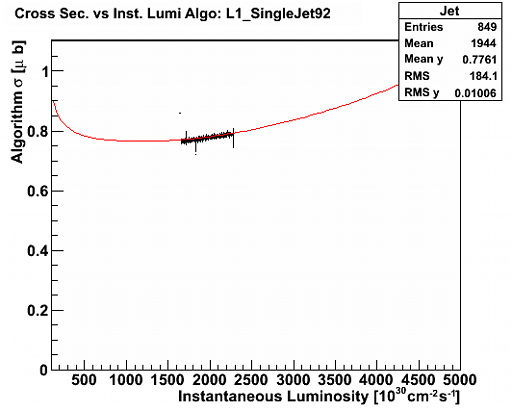
\includegraphics[width=0.45\textwidth]{Chapter03/L1TOnline/Images/Run177878_Jet_CrossSection.png}
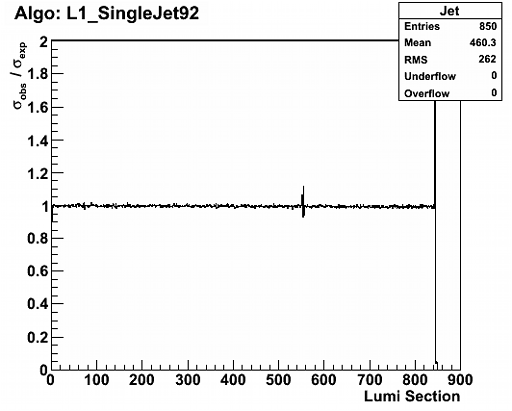
\includegraphics[width=0.45\textwidth]{Chapter03/L1TOnline/Images/Run177878_Jet_RateCertification.png}
\caption{Monitoring plot produced by the L1TRate tool for L1 $E_T^{miss}$ object category, which is automatically
monitoring algorithm L1\_ETM50 for the run 207099. In the plots data points are the calculated trigger cross
section as a function of instant luminosity and the line is the reference fit done from previous runs.}
\label{figure_ServiceWork_L1TRate}
\end{figure}

%%%%%%%%%%%%%%%%%%%%%%%%%%%%%%%%%%%%%%%%%%%%%%%%%%%%%%%%%%%%%%%%%%%%%%%%%%%%%%%%%%%%%%%
%%% SUBSECTION
%%%%%%%%%%%%%%%%%%%%%%%%%%%%%%%%%%%%%%%%%%%%%%%%%%%%%%%%%%%%%%%%%%%%%%%%%%%%%%%%%%%%%%%
\subsection{Synchronization Monitoring}

%Status: Writting

This tool was initially developed by me during last year and now has been improved and debugged. It monitors
the synchronization of the lowest unprescaled single object trigger of all available L1 trigger object categories
by looking at \gls{HLT} pass-through paths events (no selection at \gls{LHC} to avoid bias) and looking at the 5 bunch crossing
L1 trigger information provided by the GT. The trigger records can then be compared with the published LHC bunch
structure and a fraction of in time events can be calculated. New developments include alteration in the way
information is retrieved from the database and avoiding the use of \gls{HLT} pass-throughs and therefore improving statistics
by looking at events from an object category seeded by an independent object category. As an example: single muon
trigger can seed calorimeter triggers synchronization tests.

\begin{figure}[!htb]
\centering
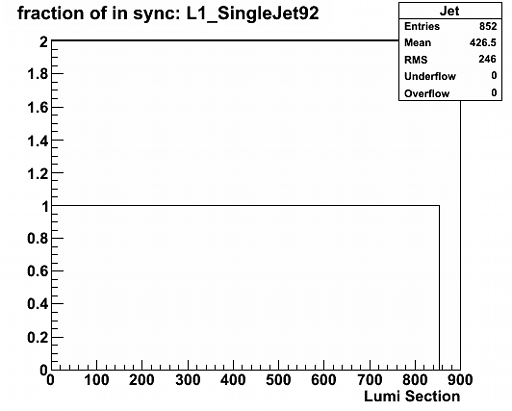
\includegraphics[width=0.45\textwidth]{Chapter03/L1TOnline/Images/Run177878_Jet_SynchronizationCertification.png}
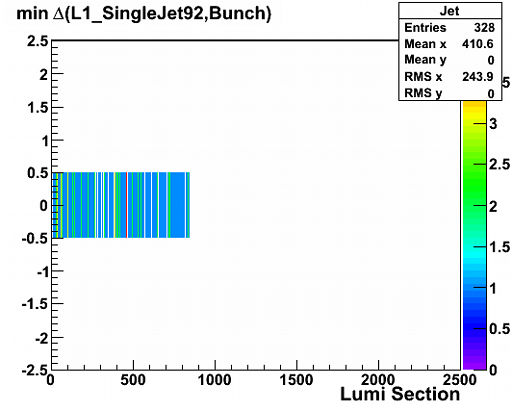
\includegraphics[width=0.45\textwidth]{Chapter03/L1TOnline/Images/Run177878_Jet_SynchronizationTest.png}
\caption{Monitoring plot produced by the L1TSync tool for L1 single electron/gamma object category, which is
automatically monitoring algorithm L1\_SingleEG50 for the run 177878. In the plots data points are the calculated
trigger cross section as a function of instant luminosity and the line is the reference fit done from previous runs.}
\label{figure_ServiceWork_L1TSync}
\end{figure}

%%%%%%%%%%%%%%%%%%%%%%%%%%%%%%%%%%%%%%%%%%%%%%%%%%%%%%%%%%%%%%%%%%%%%%%%%%%%%%%%%%%%%%%
%%% SUBSUBSECTION
%%%%%%%%%%%%%%%%%%%%%%%%%%%%%%%%%%%%%%%%%%%%%%%%%%%%%%%%%%%%%%%%%%%%%%%%%%%%%%%%%%%%%%%
\subsubsection{BPTX Monitoring}

%Status: Writting

This tool was created during August 2012 to meet a concern of the \gls{L1T} trigger management. It monitors the \gls{BPTX} system by looking at the information present at each event that 
is analyzed by the \gls{DQM} system, including the 2 bunch crossings before and after the actual event that fired. Then it 
compares where the \gls{BPTX} fired on those 5 bunch crossings with the LHC published bunch structure. The \gls{BPTX} efficiency 
and misfire rate are calculated and the rate stability is also monitored.

%%%%%%%%%%%%%%%%%%%%%%%%%%%%%%%%%%%%%%%%%%%%%%%%%%%%%%%%%%%%%%%%%%%%%%%%%%%%%%%%%%%%%%%
%%% SUBSECTION
%%%%%%%%%%%%%%%%%%%%%%%%%%%%%%%%%%%%%%%%%%%%%%%%%%%%%%%%%%%%%%%%%%%%%%%%%%%%%%%%%%%%%%%
\subsection{Implementation Tests}

%Status: Writting

\begin{figure}[!htb]
\centering
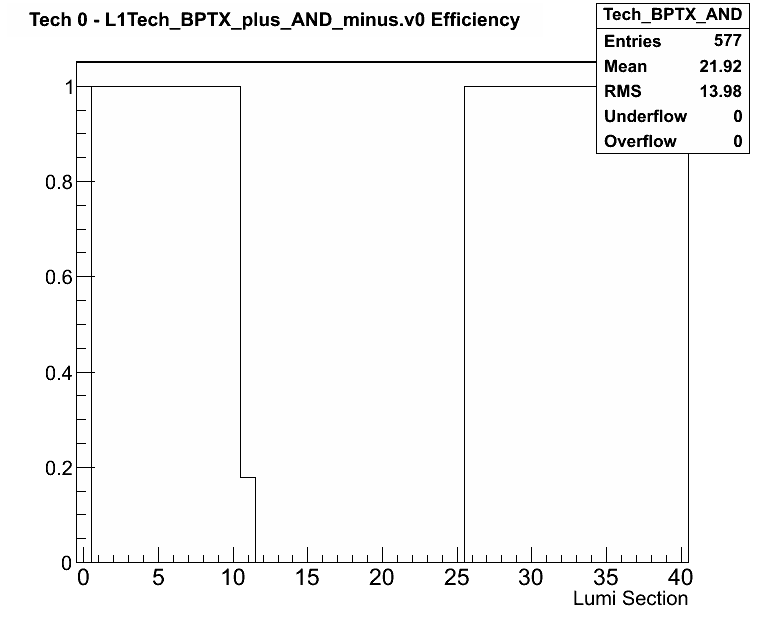
\includegraphics[width=0.45\textwidth]{Chapter03/L1TOnline/Images/L1TBPTX_Tech_BPTX_AND.png}
\caption{Monitoring plot produced by the L1TBPTX tool for the run 207269 where a test was executed to demonstrate that 
this tools works. In the plot the BPTX AND (technical algorithm 0) efficiency is calculated per luminosity section 
when compared with the LHC published bunch structure. The dip in efficiency corresponds to the disabling of the BPTX 
related triggers.} 
\label{figure_ServiceWork_L1TBPTX}
\end{figure}

%%%%%%%%%%%%%%%%%%%%%%%%%%%%%%%%%%%%%%%%%%%%%%%%%%%%%%%%%%%%%%%%%%%%%%%%%%%%%%%%%%%%%%%
%%% SUBSECTION
%%%%%%%%%%%%%%%%%%%%%%%%%%%%%%%%%%%%%%%%%%%%%%%%%%%%%%%%%%%%%%%%%%%%%%%%%%%%%%%%%%%%%%%
\subsection{Occupancy Monitoring}

%Status: Writting

This tool was developed initially by me in collaboration with a CERN summer student during last year and has been
also improved and debugged. It monitors several key occupancy plots from L1 subsystems, by making use of the natural
$\eta-\phi$ symmetry normally present. It compares each cell to the median of a strip in $\phi$ in the opposite $\eta$
side of the detector, by applying a $\chi^{2}$ like test tuned to fire when the cell is less than 10\% or more than
twice the value of the reference median. New developments include the inclusion of new plots which comply with the
tools specifications (provided by the sub-systems) and include the possibility of masking strips from the test, which 
will make the tool compare the cell with the median of the $\phi$ strip where it is included.

\begin{figure}[!htb]
\centering
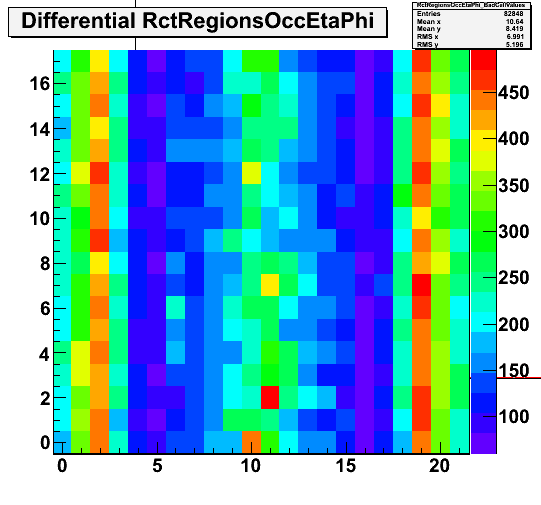
\includegraphics[width=0.45\textwidth]{Chapter03/L1TOnline/Images/L1TOccupancy_Diff.png}
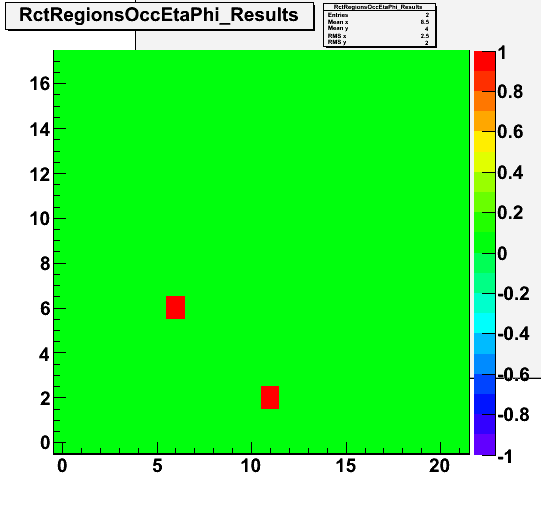
\includegraphics[width=0.45\textwidth]{Chapter03/L1TOnline/Images/L1TOccupancy_Results.png}
\caption{Monitoring plot produced by the L1TOccupancy tool for the run 207099 while testing GCT plot for isolated
EM occupancy $\eta-\phi$. In blue are the masked bins, in green the cells that pass the test and in red the cells
that fail the test. The cells marked as bad are in fact a consequence of the initial plot being produced without
a cut on minimum $p_T$ on the trigger primitives, so the asymmetries observed are due to pedestal differences between
difference areas.}
\label{figure_ServiceWork_L1TOccupancy}
\end{figure}

\section{Status Summary Display}

%Status: Writting

\begin{figure}[!htb]
\centering
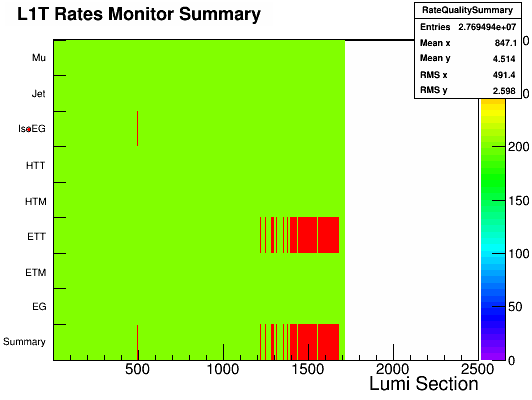
\includegraphics[width=0.45\textwidth]{Chapter03/L1TOnline/Images/RateQualitySummary.png} 
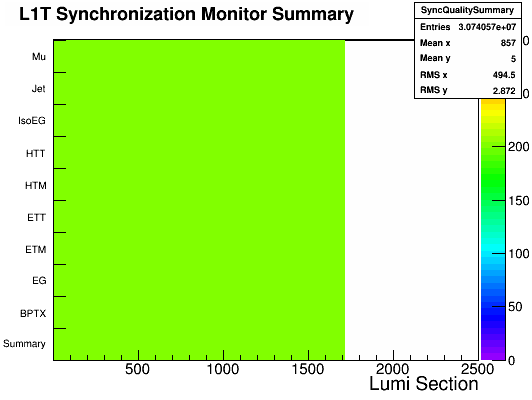
\includegraphics[width=0.45\textwidth]{Chapter03/L1TOnline/Images/SyncQualitySummary.png} \\
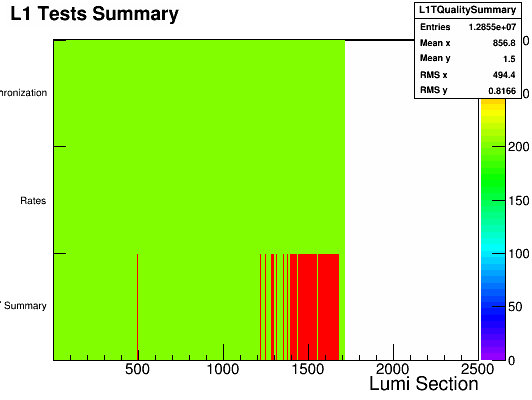
\includegraphics[width=0.45\textwidth]{Chapter03/L1TOnline/Images/L1TQualitySummary.png}
\caption{}
\label{figure_ServiceWork_StatusSummary}
\end{figure}

%%%%%%%%%%%%%%%%%%%%%%%%%%%%%%%%%%%%%%%%%%%%%%%%%%%%%%%%%%%%%%%%%%%%%%%%%%%%%%%%%%%%%%%
%%% SUBSECTION
%%%%%%%%%%%%%%%%%%%%%%%%%%%%%%%%%%%%%%%%%%%%%%%%%%%%%%%%%%%%%%%%%%%%%%%%%%%%%%%%%%%%%%%
\subsection{Certification}

%Status: Writting

% \section{Proposed Future Upgrades}
